\chapter{Technical Background and Related Work}
\label{sec:state}

% Hier werden zwei wesentliche Aufgaben erledigt:

% 1. Der Leser muß alles beigebracht bekommen, was er zum Verständnis
% der späteren Kapitel braucht. Insbesondere sind in unserem Fach die
% Systemvoraussetzungen zu klären, die man später benutzt. Zulässig ist
% auch, daß man hier auf Tutorials oder Ähnliches verweist, die hier auf
% dem Netz zugänglich sind.

% 2. Es muß klar werden, was anderswo zu diesem Problem gearbeitet
% wird. Insbesondere sollen natürlich die Lücken der anderen klar
% werden. Warum ist die eigene Arbeit, der eigene Ansatz wichtig, um
% hier den Stand der Technik weiterzubringen? Dieses Kapitel wird von
% vielen Lesern übergangen (nicht aber vom Gutachter ;-), auch später
% bei Veröffentlichungen ist "Related Work" eine wichtige Sache.

% Viele Leser stellen dann später fest, daß sie einige der Grundlagen
% doch brauchen und blättern zurück. Deshalb ist es gut,
% Rückwärtsverweise in späteren Kapiteln zu haben, und zwar so, daß man
% die Abschnitte, auf die verwiesen wird, auch für sich lesen
% kann. Diese Kapitel kann relativ lang werden, je größer der Kontext
% der Arbeit, desto länger. Es lohnt sich auch! Den Text kann man unter
% Umständen wiederverwenden, indem man ihn als "Tutorial" zu einem
% Gebiet auch dem Netz zugänglich macht.

% Dadurch gewinnt man manchmal wertvolle Hinweise von Kollegen. Dieses
% Kapitel wird in der Regel zuerst geschrieben und ist das Einfachste
% (oder das Schwerste weil erste).

%\ldots state of the art \ldots

%\todo{write state}

\section{Technical Background}
In this chapter, we first introduce the privilege transition. Then we motivate our new 
design by discussing the limitations of privilege 
transition we fund. Furthermore, we provide you a general overview of 
meltdown and similar vulnerabilities since our new design is greatly 
influenced by those vulnerabilities. In the end, we survey other techniques 
aiming for high-performance IO operation.

\subsection{Privilege Transitions}
\begin{figure}[H]
  \centering
  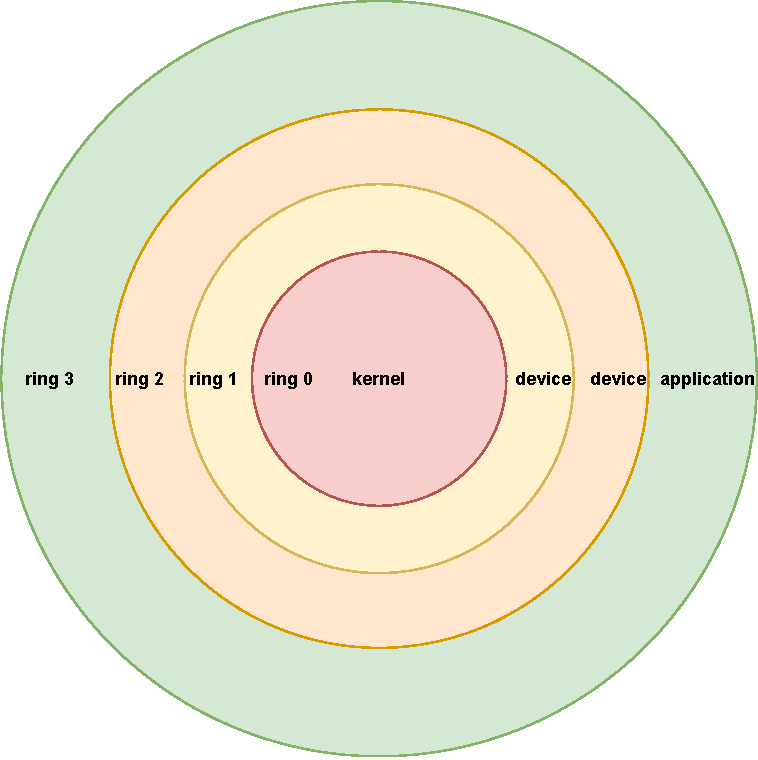
\includegraphics[width=0.8\textwidth]{images/ring_protection}
  \caption[Ring protection mechanisms]{Ring protection mechanisms}
  \label{fig:ring_protection}
\end{figure}
System calls are the most common communication method between devices and applications.  
An application can't access devices directly because device memory typically resides in 
 kernel and is protected by the ring protection.  While the ring protection provides security, 
 it forces the user-land application to do the privilege transition if the application needs to 
 manipulate a device.



 Most operating systems employ the protection ring mechanism\cite{13} to isolate user-kernel land. 
 Figure ~\ref{fig:ring_protection} provides a sketch of this mechanism. Typically, it has multiple different privilege levels, 
 ring0 to ring n. While ring 0 is the most privileged level, ring n is the least privileged
 Note that this mechanism is enforced by hardware, i.e., the CPU provides different running modes 
 to fit this mechanism.  Specifically, X86 architecture support 4 level ring mechanism, i.e., 
 ring 0 and ring 3.  Ring 0 (the kernel land)is the most privileged level, which contains critical 
 resources and sensitive data such as device memory, scheduler information, and physical memory. 
 On the contrary, ring 3 is called user land where untrusted applications/processes are running.  
 Compared to processes in ring zero that can do anything, processes in ring 3 cannot touch any 
 critical resources.


 The kernel use system calls to provide various services to user-level processes, i.e., the processes 
 can indirectly use critical resources in the kernel through system calls. This workflow has 2 major 
 advantages. First, it has improved system security. The kernel can validate requests that come from 
 user space before providing services. Therefore, a malicious process can not intentionally sabotage 
 critical resources protected by the kernel. Secondly, the combination of the ring protection 
 mechanisms and system calls gives user-level process flexibility. A user-level process does not 
 have to worry about contention with others for critical resources managed by the kernel. Because 
 it is the kernel's responsibility to determines the order in which the process uses the resource. 
 

 However, the ring mechanism also introduces a significant performance loss. 
 This is because that the user-land and kernel-land are isolated. Whenever a user-land 
 process enters the kernel land through system calls, it must cross the user-kernel boundary 
 and perform privilege transition.  The process of privilege transition is quite complex. 
 It involves multiple times saving and restoring of registers, CPU mode switch(user to privilege mode), 
 permission checking, etc. Thus, the privilege transition is very costly.

 Now, let us take a look at the system call's workflow\cite{8}. From it, you can be aware of 
 how complex and expensive the privilege transition can be.
 \begin{enumerate}
  \item User-land processes employ a wrapper function provided by the c library to invoke system calls.
  \item The arguments are passed to the wrapper function through the stack. However, the kernel requires system call arguments passing by 6 registers. Therefore, the wrapper function has to copy arguments from its stack to registers.
  \item Each system call has a unique number to identify itself from other system calls. The wrapper function needs to specify this system call number and save it in the register \%eax.
  \item The wrapper function executes the syscall instruction.  This instruction notifies the CPU to perform the mode switch(user to privilege mode) then jump to the os-level system call handler.
  \item In the handler:
  \begin{enumerate}
    \item User page table and stack are switched to kernel page table and stack.
    \item Registers are saved to the kernel stack.
    \item The system call number and arguments are validated. Then, according to the number, the handler searches the system call table place on the memory to find the corresponding system call service routine.
    \item The handler calls the system call service routine and passes the system call arguments to it.
    \item After the routine is completed, it returns the results to the handler.
    \item Registers are restored, page table and the stack are switched back.
    \item The handler returns the results and notifies the CPU to switch back to user mode.
  \end{enumerate}
  \item The wrapper function gets the returned value from the handler through the register \%rax and forwards it to the user-land process.
  
\end{enumerate}

 
 
 
 

 

 




 
 
\subsection{\emph{Meltdown} attack}

The CPU side-channel attacks such as \emph{meltdown}\cite{3} and \emph{spectre}\cite{4} are mainly based on 
CPU speculative execution and microarchitecture side channel such as caches. 
In general, accessing memory and some other operations can be expensive. 
In order to prevent the CPU from busy waiting(Pipeline stalling), 
the CPU allows instructions to execute out of order, i.e., independent 
instructions in a code snippet can be proceeded in parallel. After the out-of-order 
executed instructions are completed,  the CPU reorders them and retires(commits the 
results of the instructions) them one by one. Note that the CPU retires one instruction 
only if it is certain that all previous instructions are retired successfully, and the 
instruction has passed the permission check.  Specifically, in the context of memory access, 
the Intel CPU checks the permission control bits on the page table entry(during the 
instruction retirement stage) after it accessed the memory. 
Previously, this was considered safe since the CPU undo everything and reverts 
its state if the permission check fails.
However, clever attackers find out that the CPU does not actually clear all the 
failed instruction's effects on computer microarchitecture. For instance, 
the record in the cache is not cleared if memory access-related instruction 
fails because of the page table permission check. Thus, an attacker can employ 
\emph{clflush} instruction to flush the cache in advance then lets the CPU speculatively 
executes an instruction that reads a secret. Finally, the attacker can get the secret 
by timing the cache(flush and reload\cite{11}).

Now let us view a code snippet from MIT 6.828\cite{1}, which shows how meltdown works. Note here we assume that the user space and the 
kernel space share one page-table. 
\begin{lstlisting}[style=CStyle]
  char buf[8192]

  // the Flush of Flush+Reload
  clflush buf[0]
  clflush buf[4096]

  <some expensive instruction like divide>

  r1 = <a kernel virtual address>
  r2 = *r1
  r2 = r2 & 1      // speculated
  r2 = r2 * 4096   // speculated
  r3 = buf[r2]     // speculated

  <handle the page fault from "r2 = *r1">

  // the Reload of Flush+Reload
  a = rdtsc
  r0 = buf[0]
  b = rdtsc
  r1 = buf[4096]
  c = rdtsc
  if b-a < c-b:
    low bit was probably a 1
\end{lstlisting}

In this code snippet, an attacker exploits the out-of-order execution and 
microarchitecture side channel to read the secret out of kernel memory. 
The attacker first allocates a buffer with 8192 bytes. Then the attacker uses 
\emph{clflush} to clear any records related to \emph{buf[0]} and \emph{buf[4096]} in the cache. 
Next, we let the CPU execute a costly instruction that may take more than 1000 cycles. 
In order to prevent any performance loss, instead of waiting for the completion of the instruction,  
the CPU(multi-cores) speculatively execute the following instructions(line 11-13). 
Because those instructions are executed out of order, the CPU chooses to run them and does 
not care whether the current process has permission to access this kernel memory. 
After the CPU completes the CPU in line 13, the CPU decides to reorder all speculatively 
executed instructions and retires them one by one. At this point, the CPU finally 
realizes that the current process does not have permission to access kernel memory 
according to PTE\_U (the page table entry user bit), then reverts the state of itself. 
However, the result of the instruction \emph{r3 = buf[r2]} has already been cached. Therefore, 
the attacker can guess the first bit of the kernel address through cache timing\cite{11}. 

Since the meltdown is a hardware-based vulnerability, it is hard to prevent the attacker 
from exploiting it. One intermediate solution is KPTI\cite{2}, which separates the original page 
table into two page-tables, i.e., user and kernel page table.  While the kernel page table 
contains all sensitive data, each user page table only includes the data belonging to one process. 
In this case, the instruction(line 10) in the above code snippet would cause a segfault if 
a process tries to run the code on its user space. Because the user page table does not contain 
the mapping between the kernel virtual address in r1 and the physical address anymore. Therefore, 
a malicious process can not read any secret in the kernel through meltdown anymore. However, 
it also brings overhead when operations like system calls need to cross the user-kernel boundary 
since the page table must be switched back and forth.

\subsection{\emph{Spectre} attack}

\emph{Spectre}\cite{4} is similar to meltdown vulnerability. It also bases on speculative 
execution and microarchitecture side channel such as caches. However, unlike meltdown the 
\emph{Spectre} attack manipulates a unit in the CPU called branch predictor to execute some wrong 
code that can steal secrets.  The branch predictor can generally be used in 3 places\cite{5}:



\begin{enumerate}
  \item The branch direction prediction,  such as if(valid).
  \item The branch target prediction, such as jmp [eax].
  \item The return stack buffer, such as instruction return.
\end{enumerate}
In the following description, we use branch direction prediction as an example to show 
how \emph{Spectre} works.  Specifically, there are 2 different methods to exploit the branch 
predictor during the branch prediction.  In the first method, the attacker first mistrains 
the predictor by executing some branches intentionally.  In this case, many wrong records 
are written into the branch predictor. Then the attacker executes a carefully selected branch. 
Due to the branch predictor mistraining, the predictor may choose the wrong branch to do 
speculative execution.  In the wrong branch, secrets can be read out of memory and cached. 
Later, the attacker can get the secrets through cache timing\cite{11}.

In the second method, 
because the branch predictor is shared by all processes running on the same core, 
a malicious process can write wrong samples into the predictor so that the victim process will 
jump to a carefully selected code snippet(the gadget) through a wrong branch prediction. 
After the execution of the gadget, secrets can be cached into the cache. Later, the attacker 
can get the secrets through cache timing.

\section{Related work}
The IO stands for data transformation between user-level processes 
and various devices. A complete IO is usually divided into 2 phases:
\begin{itemize}
  \item Privilege transitions between user space and kernel space.
  \item Communication between kernel space and device space.
\end{itemize}  
In recent years, with the continuous improvement of device IO speed, 
The IO operations' overhead in the kernel has become not negligible anymore. 
To address this issue, clever developers proposed many approaches. 
This section will cover some of them, which aim to alleviate the IO 
performance bottleneck caused by the kernel.

\subsection{vDSO}

Let us first look at \emph{vDSO}\cite{9}. \emph{vDSO} stands for Virtual Dynamic Shared Object, 
which accelerates some read-only system calls by mapping pages containing 
relevant information and codes to user space. In particular, the pages are 
mapped both to user and kernel space. While the page in the kernel is writable, 
the mapping containing the page in user space is read-only, 
and the mapping address is randomized against the attacker.  
\emph{vDSO} improves IO performance, but it also has obvious limitations. 
That is, all codes and data related to \emph{vDSO} in the user space are read-only. 
If the program wants to transfer data to the device, it can only enter the 
kernel or try other methods. Therefore, \emph{vDSO} is still regarded as an 
IO slow path in the context of the communication  between the application 
and the device,
\subsection{io\_uring}
\begin{figure}[tbp]
  \centering
  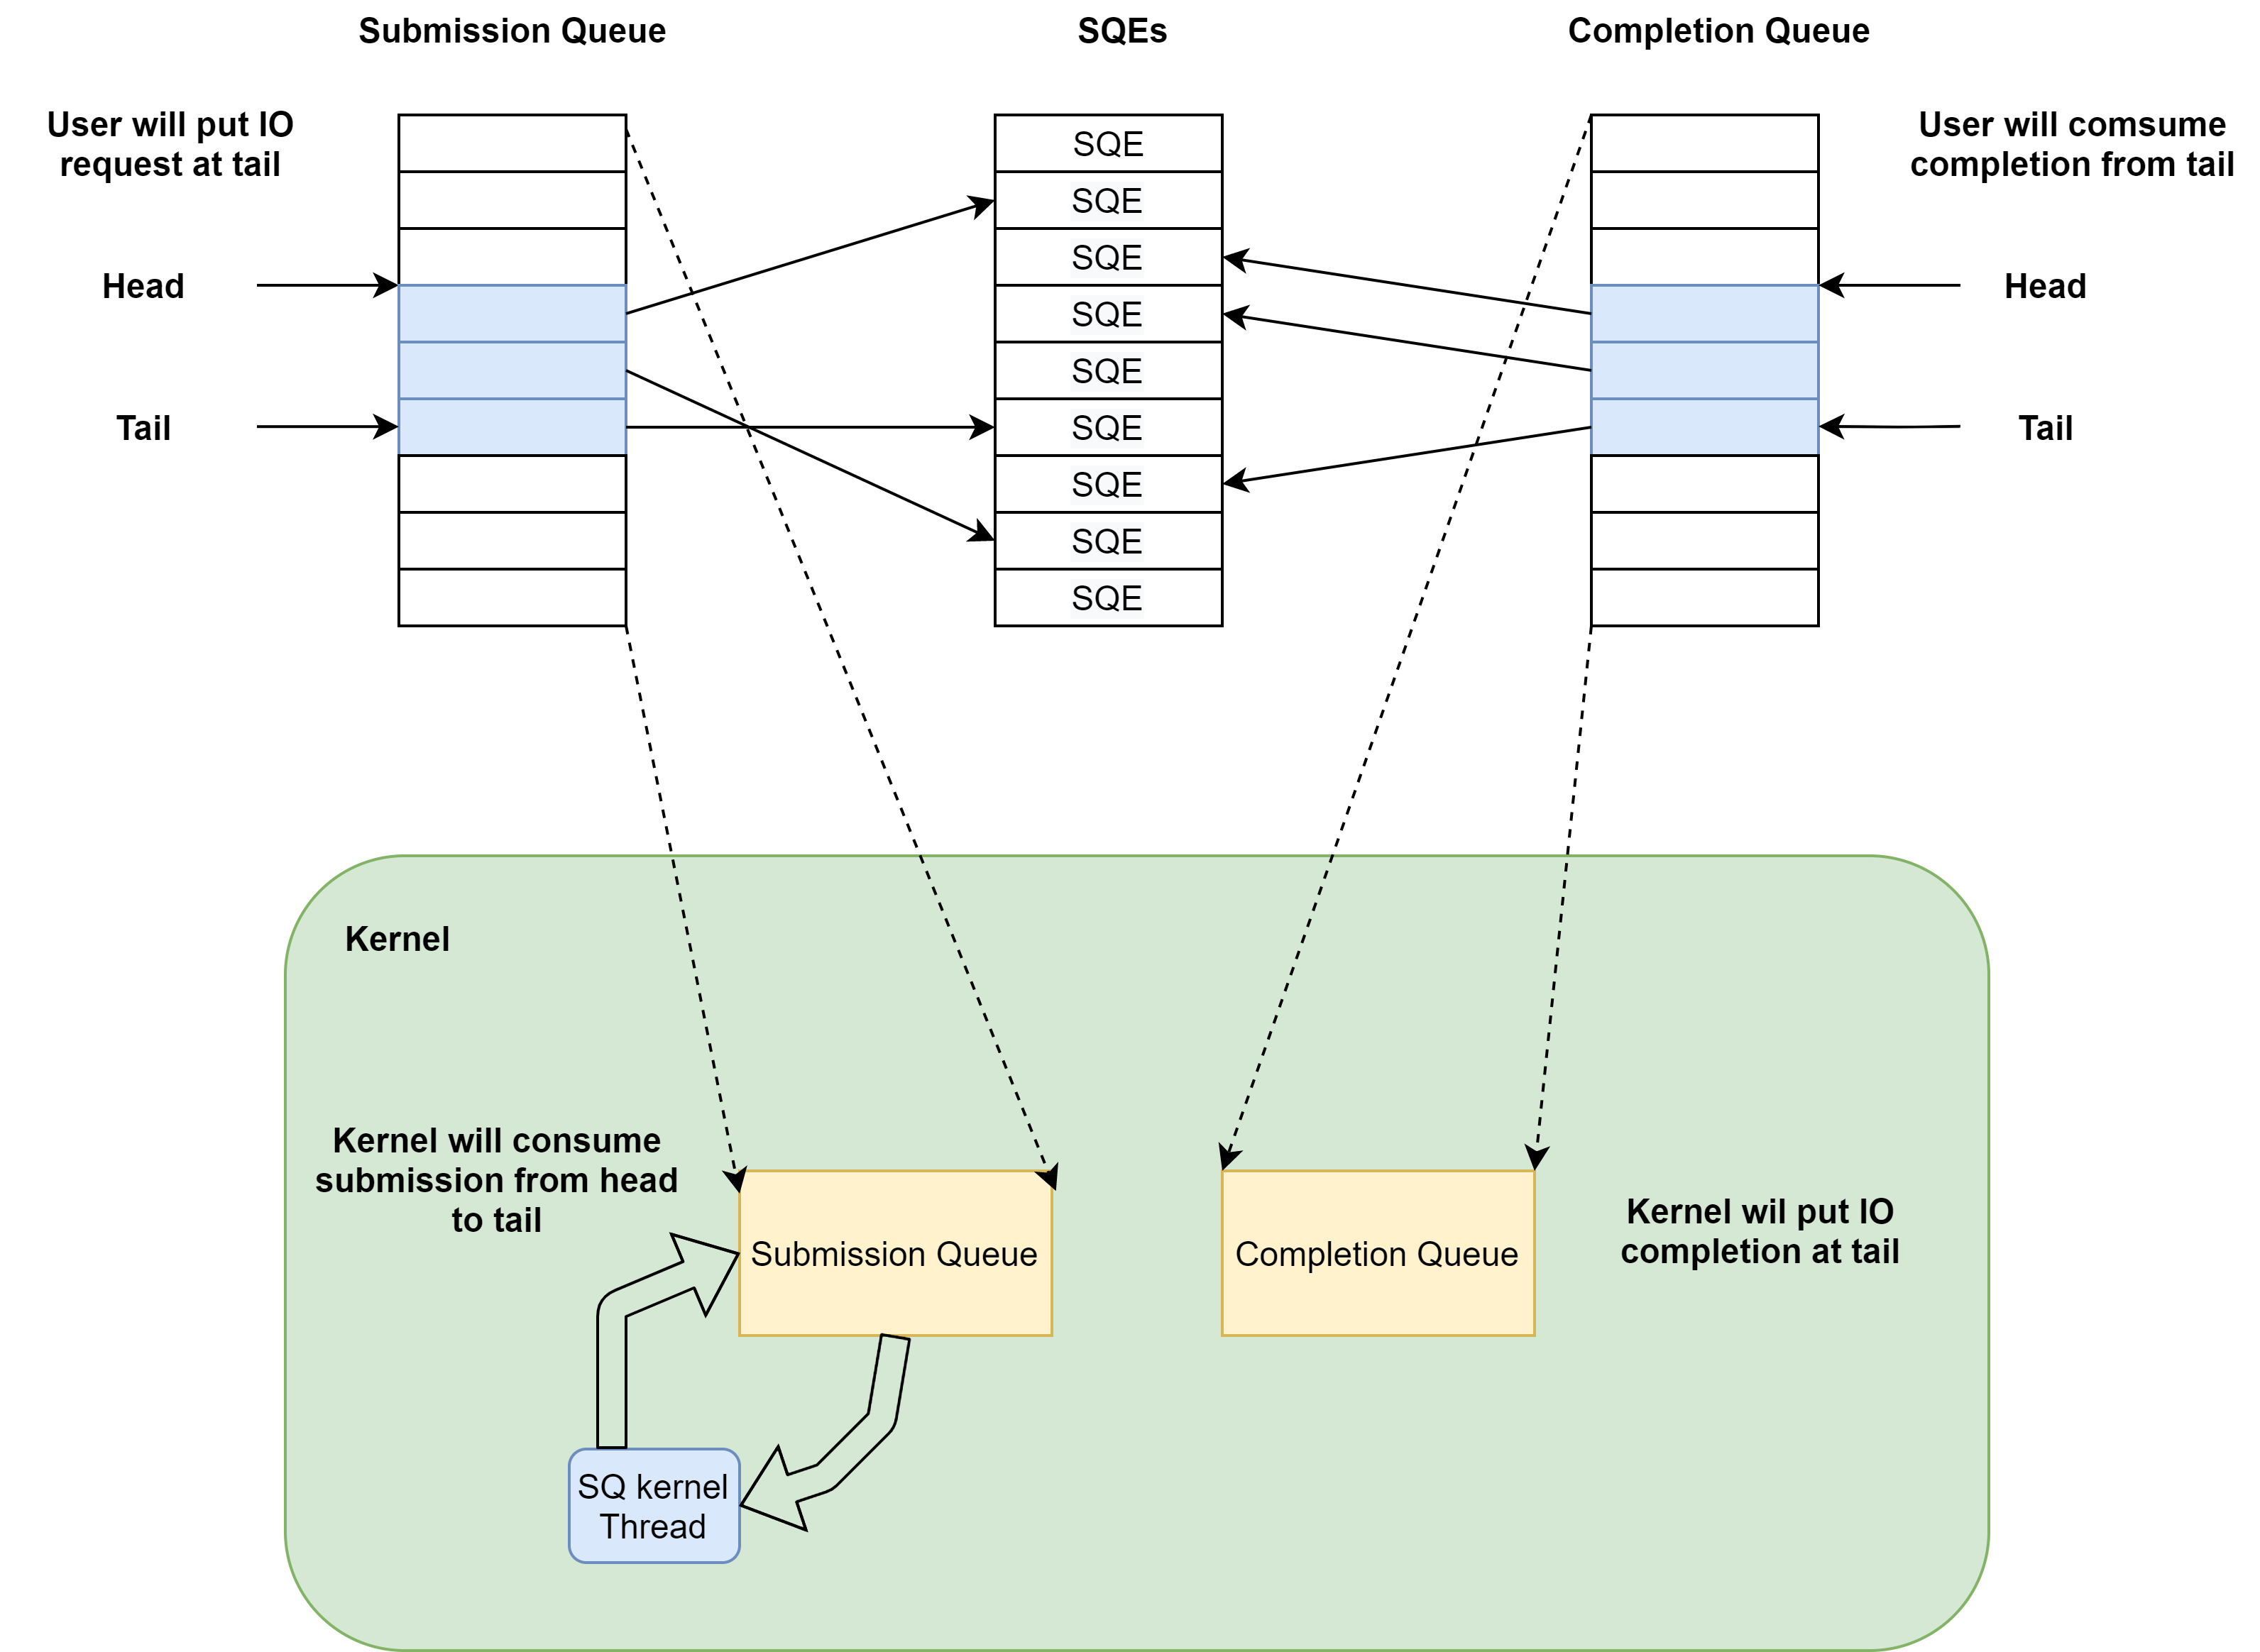
\includegraphics[width=0.8\textwidth]{images/IOURING}
  \caption[io\_uring]{io\_uring}
  \label{fig:IOURING}
\end{figure}

\emph{io\_uring}\cite{10} is introduced in Linux version 
5.1 and refers to a new generation of asynchronous 
I/O API. It offers batch processing and asynchronous 
I/O submission/completion,  reducing the pressure caused 
by the user-kernel boundary-crossing and eliminating 
it in the best case. This is done by entering the fully 
polled mode that enables a \emph{SQ kernel thread} to poll the 
submission queue and to submit any requests found there 
automatically. In detail, \emph{io\_uring} has three essential 
components in the fully polled mode. Those are \emph{submission queue}, 
\emph{completion queue}, and \emph{SQ kernel thread} as despite in Figure 
~\ref{fig:IOURING}.  A user-level process needs to do three system calls 
to map \emph{Submission Queue}, \emph{Completion Queue}, and 
\emph{Submission Queue Entries} ( SQEs ) into user space in the preparation stage. Submission Queue, 
Completion Queue is a ring buffer, which contains pointers to 
\emph{SQE} in \emph{SQEs}. As for \emph{SQE}, it contains either the uncompleted or completed 
IO request. Then the user-level process can directly put the IO request 
into \emph{SQ}and get the completed IO request from \emph{CQ}. In kernel, 
the \emph{SQ kernel thread} poll the \emph{SQ}, sends any requests it finds in the queue 
to kernel handler functions, and pushes any completed request to \emph{CQ}. 

With the help of shared queues between user and kernel space, 
\emph{io\_uring} eliminates the user kernel boundary-crossing for every
 IO request. This has resulted in a noticeable performance improvement. 
 However, during the \emph{io\_uring} setup stage, \emph{io\_uring} 
 needs at least three system calls(6 context switches). In addition, each IO request still 
 needs to go through multiple layers in the kernel to reach the device. 
 For instance, a storage-related IO must pass through at least the file 
 system layer to arrive at the appropriate device driver layer. Hence, 
 each IO operation still brings noticeable overhead.
\subsection{OS-bypass}
\begin{figure}[tbp]
  \centering
  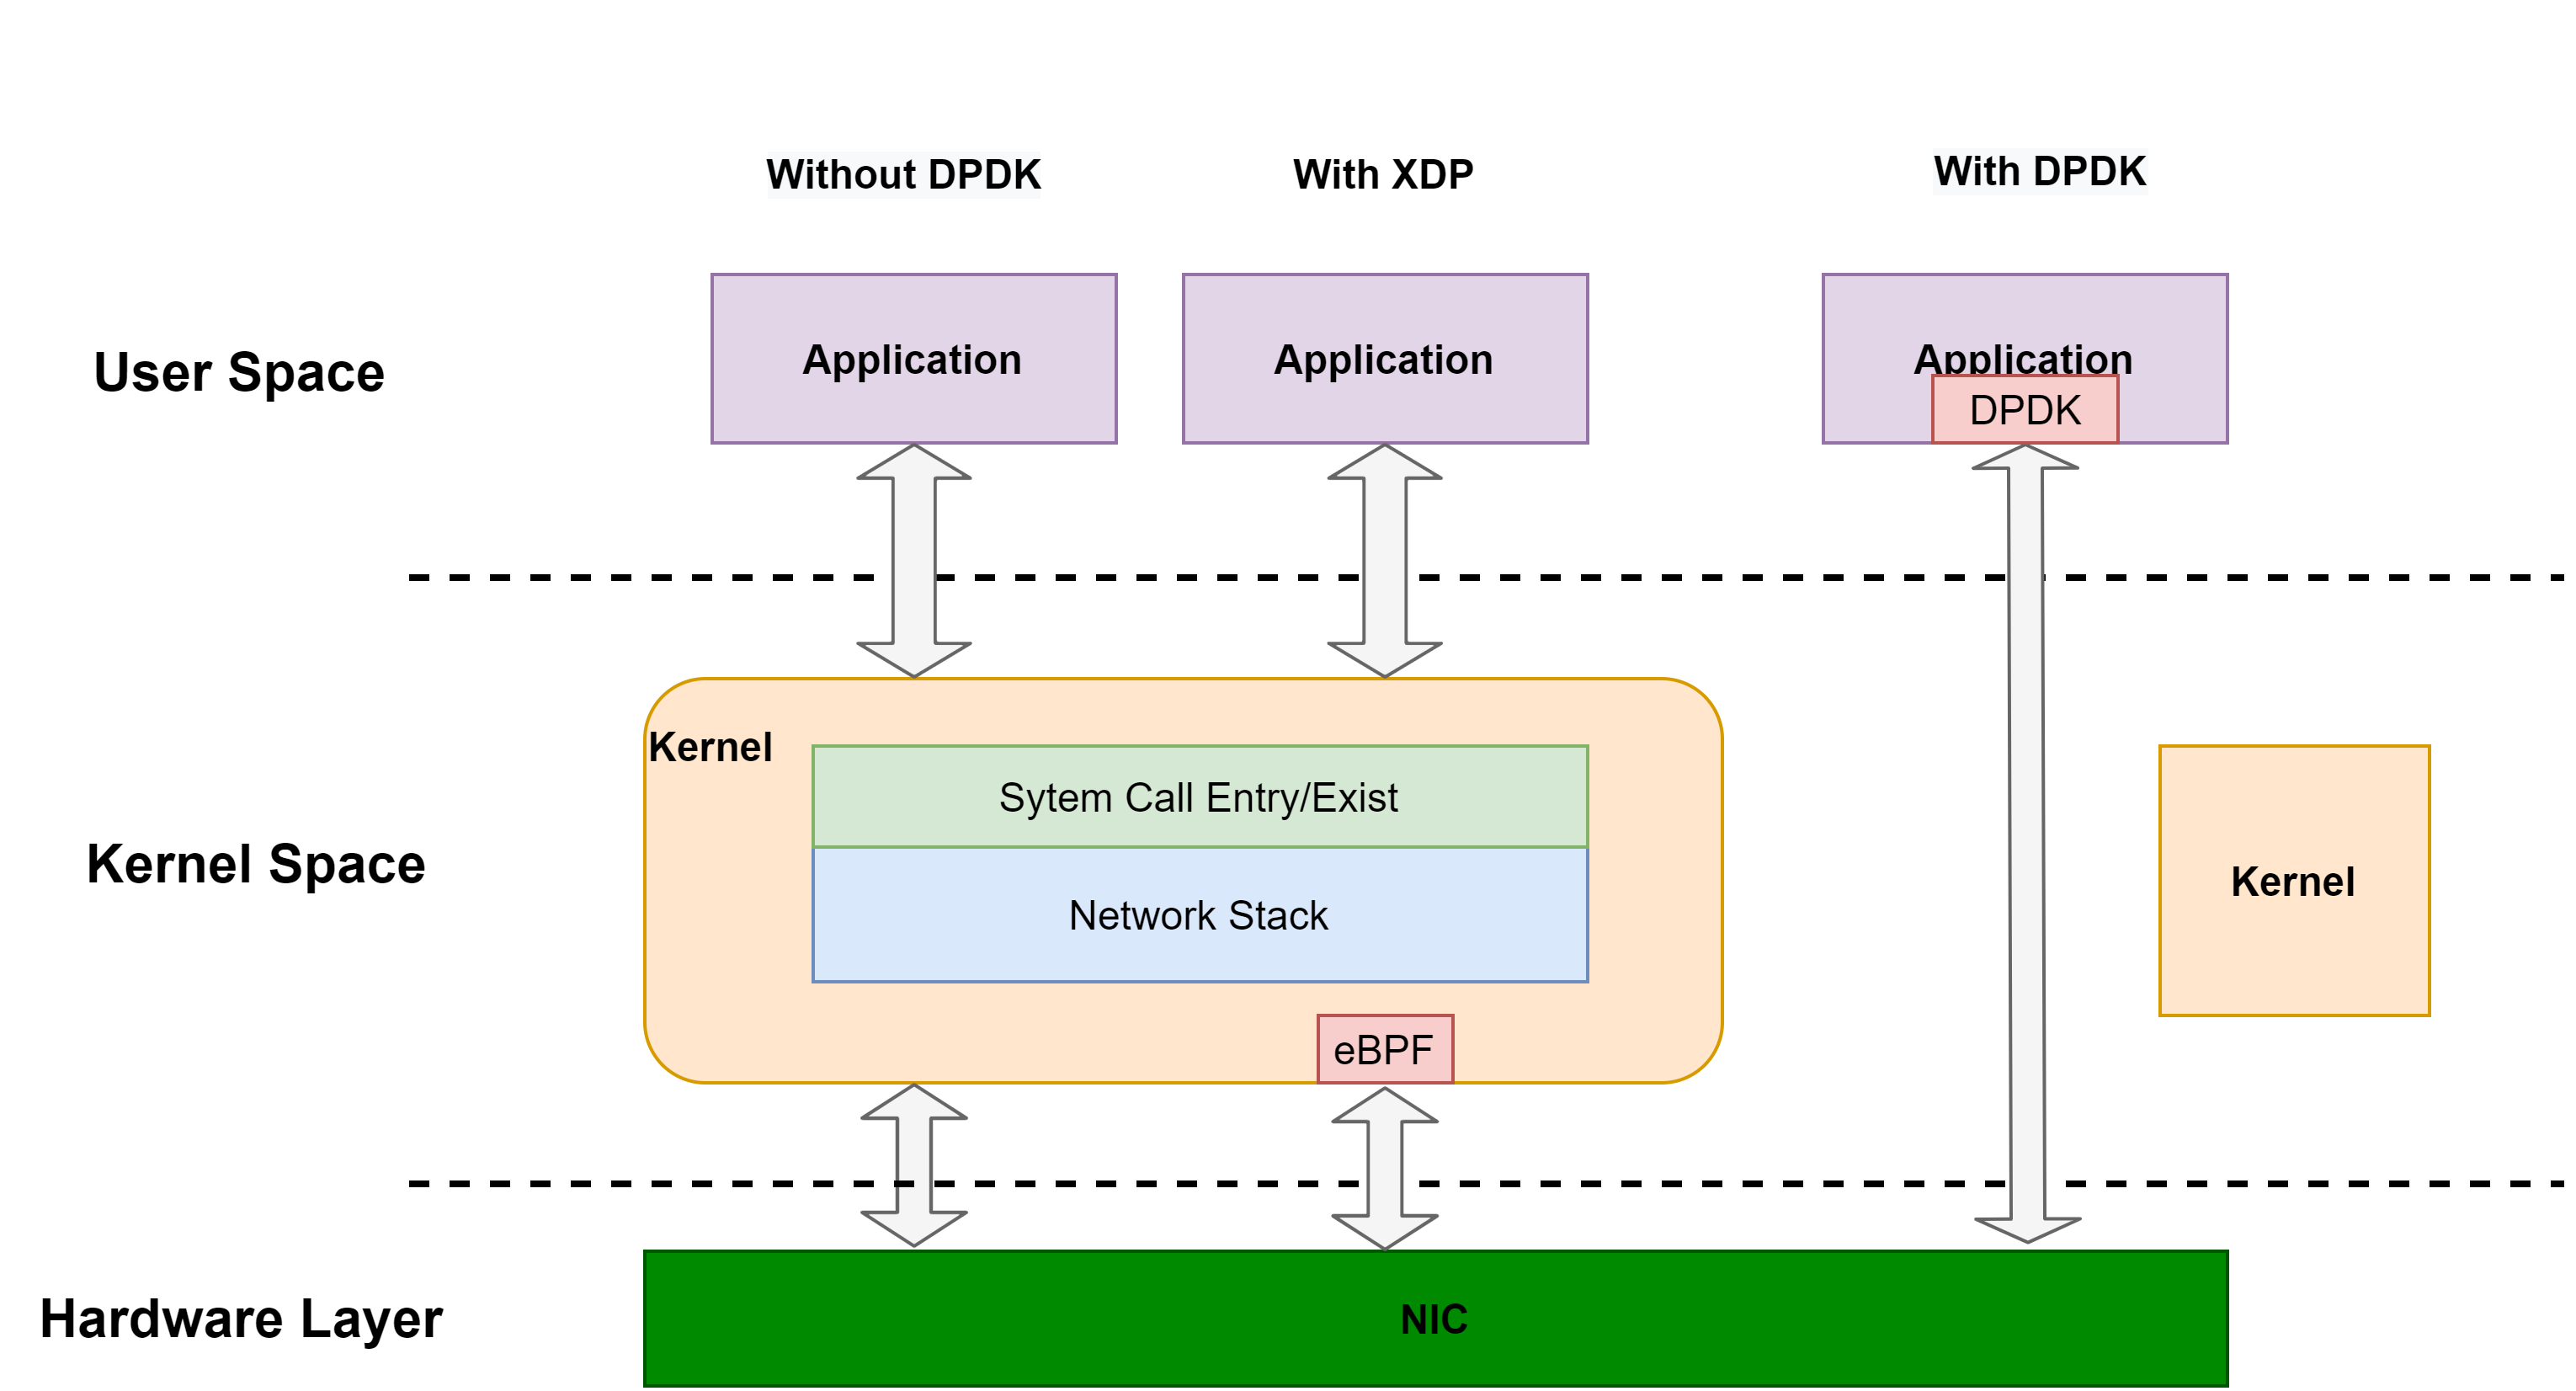
\includegraphics[width=0.8\textwidth]{images/Linux_networking}
  \caption[Linux Networking]{Linux Networking}
  \label{fig:Linux_networking}
\end{figure}



Kernel bypass, such as \emph{DPDK}\cite{7} (for intelligent network cards), allows applications to communicate 
with devices without involving the kernel. For example, as shown 
in Figure ~\ref{fig:Linux_networking}, in the context of a 
DPDK-driven network process, the Kernel Bypass allows applications 
to bypass the kernel and process network packets on user space. In addition, 
the device registers are mapped directly to user space. 
Therefore, the application can control devices without 
any performance loss caused by privilege transition. 
It avoids multiple data copies in the kernel-oriented network 
processing, i.g., the copy between hardware and kernel and the 
copy between kernel to user space. As a result, \emph{DPDK} brings high 
throughput and low latency packet processing to applications 
compared to the Linux networking stack.

On the other hand, OS-bypass is less flexible to adapt than traditional approaches. It was 
hard to integrate with the existing OS since it has 
changed the operating mode of the current OS. 
In addition, It requires an application to implement its 
package processing library since the packages passed to 
user-land through \emph{DPDK} are raw packages. This may lead to 
a significant overhead for application developers. 
The most painful thing is that kernel bypass breaks 
the isolation between a user-land application and devices
 provided by the kernel because device registers are mapped to
 s user space directly by \emph{DPDK}.

All in all, Kernel bypass eliminates the performance 
loss in the kernel networking stack. Still, it also has 
drawbacks, such as significant application-level changes, 
lack of isolation between devices and applications, etc.

\subsection{XDP}
\emph{XDP}\cite{10.1145/3281411.3281443} stands for \emph{eXpress Data Path}, which is the opposite of 
kernel bypass technology because it has been completely embedded 
in the kernel. As shown in Figure ~\ref{fig:Linux_networking}, 
it uses \emph{eBPF} technology to place user-defined code(UDC) at the 
bottom of the kernel network stack, that is, between the kernel 
network stack and the network card. 
Data packets can be processed as soon as they arrive at the kernel 
instead of being passed to applications. The UDC can decide how to 
process the arriving data packets. For example, 
discard the data packet, forward it to other network 
routes, or send it to the kernel network stack for further processing.

In summary, by embedding the code into the kernel, 
\emph{XDP} has significantly improved the package processing 
efficiency and reduced package processing's pressure 
in the kernel. Especially \emph{XDP} does not break the isolation 
between user and kernel. Thus, it Fully ensures the safety of the device.

\cleardoublepage

%%% Local Variables:
%%% TeX-master: "diplom"
%%% End:
